\documentclass{article}
\usepackage{amsfonts, amsthm, amsmath, amssymb, mathtools, ulem, mathrsfs, physics, esint, siunitx, tikz-cd}
\usepackage{pdfpages, fullpage, color, microtype, cancel, textcomp, markdown, hyperref, graphicx}
\usepackage{enumitem}
\usepackage{algorithm}
\usepackage{algpseudocode}
\graphicspath{{./images/}}
\usepackage[english]{babel}
\usepackage[autostyle, english=american]{csquotes}
\MakeOuterQuote{"}
\usepackage{xparse}
\usepackage{tikz}

\usepackage{calligra}
\DeclareMathAlphabet{\mathcalligra}{T1}{calligra}{m}{n}
\DeclareFontShape{T1}{calligra}{m}{n}{<->s*[2.2]callig15}{}
\newcommand{\script}[1]{\ensuremath{\mathcalligra{#1}}}
\newcommand{\scr}{\script r}

% fonts
\def\mbb#1{\mathbb{#1}}
\def\mfk#1{\mathfrak{#1}}
\def\mbf#1{\mathbf{#1}}
\def\tbf#1{\textbf{#1}}

% common bold letters
\def\bP{\mbb{P}}
\def\bC{\mbb{C}}
\def\bH{\mbb{H}}
\def\bI{\mbb{I}}
\def\bR{\mbb{R}}
\def\bQ{\mbb{Q}}
\def\bZ{\mbb{Z}}
\def\bN{\mbb{N}}

% brackets
\newcommand{\br}[1]{\left(#1\right)}
\newcommand{\sbr}[1]{\left[#1\right]}
\newcommand{\brc}[1]{\left\{#1\right\}}
\newcommand{\lbr}[1]{\left\langle#1\right\rangle}

% vectors
\renewcommand{\i}{\hat{\imath}}
\renewcommand{\j}{\hat{\jmath}}
\renewcommand{\k}{\hat{k}}
\newcommand{\proj}[2]{\text{proj}_{#2}\br{#1}}
\newcommand{\m}[2][b]{\begin{#1matrix}#2\end{#1matrix}}
\newcommand{\arr}[3][\sbr]{#1{\begin{array}{#2}#3\end{array}}}

% misc
\NewDocumentCommand{\seq}{O{n} O{1} O{\infty} m}{\br{#4}_{{#1}={#2}}^{#3}}
\NewDocumentCommand{\app}{O{x} O{\infty}}{\xrightarrow{#1\to#2}}
\newcommand{\sm}{\setminus}
\newcommand{\sse}{\subseteq}
\renewcommand{\ss}{\subset}
\newcommand{\vn}{\varnothing}
\newcommand{\lc}{\epsilon_{ijk}}
\newcommand{\ep}{\epsilon}
\newcommand{\vp}{\varphi}
\renewcommand{\th}{\theta}
\newcommand{\cjg}[1]{\overline{#1}}
\newcommand{\inv}{^{-1}}
\DeclareMathOperator{\im}{im}
\DeclareMathOperator{\id}{id}
\newcommand{\ans}{\tbf{Ans. }}
\newcommand{\pf}{\tbf{Pf. }}
\newcommand{\imp}{\implies}
\newcommand{\impleft}{\reflectbox{$\implies$}}
\newcommand{\ck}{\frac1{4\pi\ep_0}}
\newcommand{\ckb}{4\pi\ep_0}
\newcommand{\sto}{\longrightarrow}
\DeclareMathOperator{\cl}{cl}
\DeclareMathOperator{\intt}{int}
\DeclareMathOperator{\bd}{bd}
\DeclareMathOperator{\Span}{span}
\newcommand{\floor}[1]{\left\lfloor#1\right\rfloor}
\newcommand{\ceil}[1]{\left\lceil#1\right\rceil}
\newcommand{\fxn}[5]{#1:\begin{array}{rcl}#2&\longrightarrow & #3\\[-0.5mm]#4&\longmapsto &#5\end{array}}
\newcommand{\sep}[1][.5cm]{\vspace{#1}}
\DeclareMathOperator{\card}{card}
\renewcommand{\ip}[2]{\lbr{#1,#2}}
\renewcommand{\bar}{\overline}
\DeclareMathOperator{\cis}{cis}
\DeclareMathOperator{\Arg}{Arg}
\newcommand{\ptl}{\partial}
\newcommand{\Om}{\Omega}

% title
\title{HW}
\author{Ryan Chen}
%\date{\today}
\setlength{\parindent}{0pt}


\begin{document}
	
\maketitle

\section*{Problem 1}

\begin{enumerate}[label=(\alph*)]
	
\item
In this part we use the fact
$$\int_{-\infty}^{\infty}\exp(-ax^2+bx)dx = \br{\frac\pi a}^{1/2}\exp[\frac{b^2}{4a}]$$
Take the Fourier transform of the PDE in $x$, using the fact $\hat{\ptl_x^n\psi}=(i\xi)^n\psi$.
$$\hat\psi_t = \frac i2(i\xi)^2\hat\psi = -\frac i2\xi^2\hat\psi
\imp \hat\psi(\xi,t) = \hat\psi_0(\xi)\exp[-\frac i2\xi^2t]$$
Take the inverse Fourier transform.
$$\psi(x,t) = \frac{1}{(2\pi)^{1/2}}\int_{-\infty}^{\infty} \hat\psi_0(\xi)\exp[ix\xi - \frac i2t\xi^2]d\xi$$

Take the Fourier transform of the initial condition.
\begin{align*}
	\hat\psi_0(\xi) &= \frac{1}{(2\pi)^{1/2}}\frac{1}{(2\pi \sigma_0^2)^{1/4}}\int_{-\infty}^{\infty} \exp[-\frac{x^2}{4\sigma_0^2} + ik_0x - i\xi x]dx\\
	&= \frac{1}{(2\pi)^{3/4}\sigma_0^{1/2}}\int_{-\infty}^{\infty} \exp[-\frac{x^2}{4\sigma_0^2} + i(k_0-\xi)x]dx\\
	&= \frac{1}{(2\pi)^{3/4}\sigma_0^{1/2}}\pi^{1/2}2\sigma_0\exp[-(\xi-k_0)^2\sigma_0^2]\\
	&= \frac{2^{1/4}\sigma_0^{1/2}}{\pi^{1/4}}\exp[-(\xi-k_0)^2\sigma_0^2]
\end{align*}

Then
$$\psi(x,t) = \frac{1}{(2\pi)^{1/2}}\frac{2^{1/4}\sigma_0^{1/2}}{\pi^{1/4}}\int_{-\infty}^{\infty}\exp[-\sigma_0^2(\xi-k_0)^2 - \frac i2t\xi^2 + ix\xi]d\xi$$
Rewrite the argument of exp as
$$-\sigma_0^2(\xi-k_0)^2 - \frac i2t\xi^2 + ix\xi
= -\sigma_0^2(\xi^2+k_0^2-2k_0\xi) - \frac i2t\xi^2 + ix\xi
= -\br{\sigma_0^2 + \frac i2t}\xi^2 + (ix + 2\sigma_0^2k_0)\xi - \sigma_0^2k_0^2$$
so that
\begin{align*}
	\psi(x,t) &= \frac{\sigma_0^{1/2}}{2^{1/4}\pi^{3/4}}\int^{\infty}_{-\infty}\exp[-\br{\sigma_0^2 + \frac i2t}\xi^2 + (ix + 2\sigma_0^2k_0)\xi - \sigma_0^2k_0^2]d\xi\\
	&= \frac{\sigma_0^{1/2}}{2^{1/4}\pi^{3/4}}\exp(-\sigma_0^2k_0^2)\br{\frac{\pi}{\sigma_0^2+\frac i2t}}^{1/2}\exp[\frac{-x^2 + 4\sigma_0^4k_0^2 + 4i\sigma_0^2k_0x}{4\br{\sigma_0^2 + \frac i2t}}]\\
	&= \frac{\sigma_0^{1/2}}{2^{1/4}\pi^{1/4}}\frac{1}{(\sigma_0^2+\frac i2t)^{1/2}}\exp(-\sigma_0^2k_0^2)\exp[\frac{-x^2 + 4\sigma_0^4k_0^2 + 4i\sigma_0^2k_0x}{4\br{\sigma_0^2 + \frac i2t}}]
\end{align*}


\end{enumerate}



\section*{Problem 3}

\begin{enumerate}[label=(\alph*)]
	
\item
Fix a test function $v\in H_0^1(\Omega)$. Multiply the PDE by $v$ and integrate over $\Omega$.
$$\int_\Om \ep v\Delta udx = \int_\Om (u^3-u)vdx$$
Using Green's first identity and the fact $v=0$ on $\ptl\Om$, the LHS is
$$\int_\Om \ep v\Delta udx = -\int_\Om \ep\grad u\cdot\grad vdx + \int_{\ptl\Om} \ep v\pdv{u}{n}ds
= -\int_\Om \ep\grad u\cdot\grad vdx$$
Then we obtain the weak formulation.
$$-\int_\Om \ep\grad u\cdot\grad vdx = \int_\Om (u^3-u)vdx
\imp \int_\Om \ep\grad u\cdot\grad vdx - \int_\Om (u-u^3)vdx = 0$$


\item e


\item
Code for problem 3:

\url{https://github.com/RokettoJanpu/Scientific-Computing-2/blob/main/FINAL%20q3.ipynb}

Below is a mesh of $\Omega$.

\begin{center}
	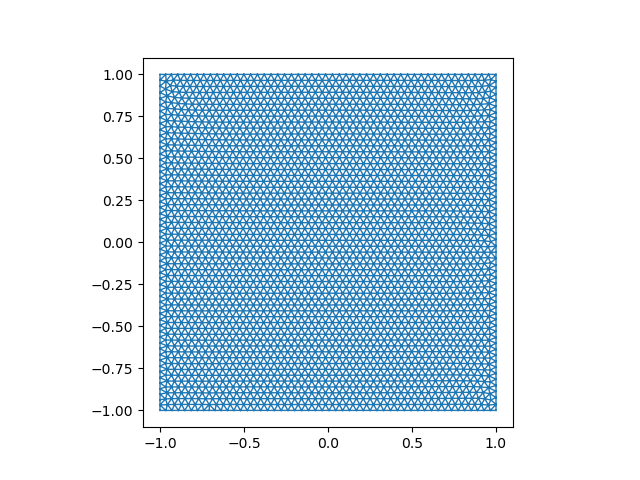
\includegraphics[scale=.5]{FINAL q3 mesh}
\end{center}
\end{enumerate}
	
\end{document}